\documentclass[11pt]{article}
\usepackage[margin=1.0in]{geometry}
\usepackage[T1]{fontenc}
\usepackage[utf8]{inputenc}
\usepackage{microtype}
\usepackage{amsmath,amssymb,amsfonts}
\usepackage{booktabs}
\usepackage{multirow}
\usepackage{graphicx}
\usepackage{xcolor}
\usepackage{hyperref}
\usepackage[numbers,sort&compress]{natbib}

\hypersetup{
  colorlinks=true,
  linkcolor=blue!55!black,
  citecolor=blue!55!black,
  urlcolor=blue!55!black
}

\newcommand{\unit}[1]{\operatorname{unit}\!\left(#1\right)}
\newcommand{\rms}[1]{\operatorname{rms}\!\left(#1\right)}
\newcommand{\sg}{\operatorname{sg}}
\newcommand{\Uphi}{U_\phi}
\newcommand{\Uval}{U_{\mathrm{val}}}
\newcommand{\Uwm}{U_{\mathrm{wm}}}
\newcommand{\Pval}{P_{\mathrm{val}}}
\newcommand{\Pwm}{P_{\mathrm{wm}}}
\newcommand{\Pfast}{P_{\mathrm{fast}}}
\newcommand{\Pslow}{P_{\mathrm{slow}}}
\newcommand{\cmeta}{c_{\mathrm{meta}}}
\newcommand{\Ksim}{K_{\mathrm{sim}}}
\newcommand{\ftd}{\textsc{FT-v3d}}
\newcommand{\fte}{\textsc{FT-v3e}}

\title{\textbf{Online Plastic World Models: Zero-Shot Test-Time Simulation Scaling, Triple-Axis Portable Plasticity, and an Equal-Compute Audit of Recursive Self-Improvement}}

\author{
  Antigravity$^{1}$\thanks{Lead AI research collaborator: architecture co-design, confirmation suites, verification, and manuscript drafting.} \quad
  Xinxin Niu$^{2}$\thanks{Project owner and corresponding human author taking scientific accountability (\texttt{xinxin.niu@outlook.com}, \url{https://cusclo.github.io/ft-v3-plastic-world-models/}).} \quad
  Claude$^{1}$ \quad
  DeepSeek$^{1}$ \quad
  GPT$^{1}$ \\[4pt]
  {\small $^{1}$AI Research Collaborators (Antigravity / Google DeepMind, Anthropic, DeepSeek, OpenAI)} \\
  {\small $^{2}$Independent Researcher, Evolve-Lab Project (\texttt{cusclo})}
}

\date{November 25, 2026}

\begin{document}
\maketitle

\begin{abstract}
Adaptive agents operating in novel environments face a fundamental tension between parameter efficiency, rapid within-trial world-model acquisition, and reliable generalization across task scales and cognitive paradigms. We present \textbf{FT-v3} (\ftd{} and its slot-attention extension \fte{}), a local plastic world-model Transformer whose cross-episode state consists solely of decoupled value ($\Pval$) and world-model ($\Pwm$) fast-slow synaptic matrices governed by triple-axis invariant local update rules $\Uphi = \{\Uval, \Uwm\}$. During zero-reward exploration, self-supervised residual prediction $\lVert \Pwm^\top k_t - \sg(s_{\text{target}}) \rVert_2^2$ in collapse-proof canonical entity coordinates writes environment transitions directly into $\Pwm$, unlocking closed-loop latent internal simulation ($\Ksim \in \{0,1,2,3\}$) without parameter retraining. Across four pre-registered, seed-isolated confirmation suites executed strictly under matched compute and deployment-level chosen-action feedback ($0$ oracle leakage): \textbf{(1) Zero-shot test-time simulation} on $6$ unseen seeds elevates greedy accuracy monotonically across out-of-distribution graph sizes and path depths ($\Ksim=0 \to 3$: \texttt{hgw8} $2$-hop $0.4368 \to 0.9531$; unseen $3$-hop $0.1155 \to 0.5397$; unseen $4$-hop $0.1043 \to 0.3777$), while \ftd{} ($374\text{k}$ params) outperforms larger full-context Transformers ($496\text{k}$, $+0.8759$) and GRUs ($550\text{k}$, $+0.8717$) $6/6$, with pure RL achieving $0.7934$ vs.\ $0.8113$ with self-imitation; \textbf{(2) Triple-axis scaling} transfers a single frozen $L{=}2, M{=}8$ rule $\Uphi^*$ at exact $0.0$ drift across $4\times$ depth ($L\in\{1,2,4\}$) and $4\times$ slot count ($M\in\{4,8,16\}$) in both key-value memory (\texttt{KV}: $+0.0877$/doubling depth, $+0.0546$/doubling slots) and hidden-graph planning (\texttt{HGW}: $+0.0514$ depth, $+0.0817$ slots), while a single $1{\times}L_4M_8$ ($640\text{k}$) model decisively defeats a parameter-larger $4{\times}L_1M_8$ ensemble ($966\text{k}$) under equal compute ($+0.2347$ on \texttt{KV}, $+0.3882$ on \texttt{HGW}, $3/3$); \textbf{(3) Cross-paradigm universality and portability} establish $4/4$ dominance of a single unmodified \ftd{} architecture across \texttt{HGW}, \texttt{KV}, selective reversal (\texttt{SR4}), and deductive code-breaking (\texttt{MM}), alongside an independent $8$-seed confirmation that rules learned on \{\texttt{HGW, KV, MM}\} transfer zero-shot to 2D multi-object \texttt{XLand-MiniGrid} when paired with \fte{} per-slot attention ($+0.0471$ vs.\ frozen $\phi_0$, $7/8$; $+0.0467$ vs.\ unfactorized \ftd{}, $8/8$; $+0.0678$ vs.\ \texttt{SLM}, $8/8$); and \textbf{(4) Equal-compute recursive self-improvement (RSI) audit} demonstrates across four multi-generation systems that apparent generational ratchets ($+0.1678$ across $G_0 \to G_3$, beating single-gen reset $+0.1194$) fail decisively ($0/3$ HURTS, $-0.1116$ to $-0.1474$) once locked-teacher (\texttt{M6}) and equal-compute continuous learners (\texttt{M7}) are evaluated, diagnosing generational $\theta$-reset exploration collapse as the underlying mechanism.
\end{abstract}

\section{Introduction}
\label{sec:intro}

Fast-weight neural architectures \citep{schmidhuber1992learning,ba2016using,miconi2018differentiable,schlag2021linear} adapt within a single lifetime by rewriting plastic associative matrices rather than relying exclusively on fixed activation states or slow outer-loop gradient updates \citep{finn2017model,wang2016learning,duan2016rl2}. While differentiable plasticity and fast-weight programmers excel at within-trial associative recall, two central limitations have restricted their generality in sequential decision making: (i) standard plasticity rules depend primarily on reward-modulated prediction errors and cannot construct an explicit dynamics model during zero-reward exploration; and (ii) coupled Transformer memory layers typically bind update-rule parameters to fixed tensor dimensions, preventing trained learning rules from transferring across model depth, memory capacity, or unseen cognitive domains.

Separately, interest in recursive self-improvement (RSI) and Expert Iteration (\textsc{ExIt}) \citep{schmidhuber2007godel,anthony2017thinking,silver2017mastering,kirsch2021meta} has produced recurring experimental designs in which an iterative multi-generation learner is compared only against its earlier generations ($G_k$ vs.\ $G_0$) or against a naive ablation whose learning rule is reset at generation $k$. Without equal-compute continuous baselines and locked-teacher controls, however, multi-generation re-distillation can generate convincing false positives.

This work resolves both challenges on a unified, local-compute-reproducible benchmark suite:
\begin{enumerate}
  \item \textbf{Online Plastic World Model \& Zero-Shot Internal Simulation (\ftd{}).} We decouple fast-slow synaptic memory into a value bank $\Pval$ and a world-model bank $\Pwm$ written via squared-$L_2$ self-supervised transition residuals against stop-gradient canonical entity coordinates $\sg(s_{\text{target}})$. Once $\Pwm$ stores transition edges during zero-reward Phase~1 exploration, closed-loop multi-hop rollouts ($\Ksim \in \{0,1,2,3\}$) scale performance monotonically on larger unseen graphs and $3$-hop / $4$-hop paths without weight retraining (\S\ref{sec:wm6}).
  \item \textbf{Triple-Axis Rule Portability \& Equal-Compute \emph{Big Apple} Scaling.} Because $\Uphi = \{\Uval, \Uwm\}$ is parameter-invariant to depth $L$, slot count $M$, and width $D$, a single static rule $\Uphi^*$ trained at $(L{=}2, M{=}8)$ transfers at $0.0$ drift across $4\times$ depth ($L \in \{1,2,4\}$) and $4\times$ slot capacity ($M \in \{4,8,16\}$), revealing clean domain-axis symmetry (\texttt{KV} depth-steeper vs.\ \texttt{HGW} slot-steeper) and decisively beating equal-compute ensembles $4\times L_1$ (\S\ref{sec:wm7}).
  \item \textbf{Cross-Paradigm Universality \& Factorized 2D Slot Portability (\fte{}).} One unmodified $374\text{k}$ \ftd{} architecture solves hidden-graph planning (\texttt{HGW}), long-horizon key-value recall (\texttt{KV}), selective reversal (\texttt{SR4}), and deductive code-breaking (\texttt{MM}), beating larger non-plastic Transformers and GRUs $4/4$ (\S\ref{sec:wm8}). Extending spatial routing to per-slot attention and full-layer write-key gradient isolation (\fte{}) cures object-attention collapse and unlocks statistically confirmed cross-paradigm $\Uphi^*$ transfer to 2D \texttt{XLand-MiniGrid} \citep{nikulin2024xland} across $8$ independent unseen seeds (\S\ref{sec:wm4c}).
  \item \textbf{Methodological Audit of RSI Mirages.} Auditing four iterative meta-learning and \textsc{ExIt} lineages (\texttt{FI1}, \texttt{P3L2B}, \texttt{FT4}, and \texttt{WM5}) reveals why generational trend, test-time reset degradation, and single-generation $\phi_0$ ablations are insufficient: when matched for total environment steps, \texttt{WM-ExIt} loses $0/3$ to both a locked teacher and a continuous single-model learner due to generational $\theta$-reset exploration collapse (\S\ref{sec:audit}).
\end{enumerate}

\section{Architecture and Method: \ftd{} and \fte{}}
\label{sec:method}

Implemented in \texttt{experiments/fruit\_jax/tf\_fruit\_v3.py}, FT-v3 processes a token sequence $O_t \in \mathbb{R}^{N_{\text{obs}} \times D}$ and discrete candidate action set $A_t \in \mathbb{R}^{C \times D}$ with validity mask $m^{\text{act}}_t \in \{0,1\}^C$ inside each trial, resetting its recurrent carry on \texttt{trial\_start}. Unlike \texttt{v2} baselines, \texttt{norew\_encoder=True} masks previous rewards from the forward stem so reward prediction error $\delta_t = [r_t - \sg(p_t),\, r_t,\, \sg(p_t)]$ enters \emph{only} the local plasticity updater $\Uphi$.

\subsection{Collapse-Proof Canonical Target Coordinates}
To prevent representation collapse during unsupervised transition learning, each valid observation token receives a static normalized attribute signature $f_{\text{tok}}(O_t) \in \mathbb{R}^{N_{\text{obs}} \times d_{\text{cue}}}$ (and role-invariant entity signature $f_{\text{ent}}(O_t)$ omitting kind biases when \texttt{sim\_coherent=True}) via fixed frozen random tables. Pre-memory spatial routing computes softmax attention weights $\alpha^{\text{pre}}_t$ from stop-gradient token embeddings $\sg(O_t)$, pooling onto a fixed constant orthonormalized projection $W_{\text{wm}} \in \mathbb{R}^{L \times M \times d_{\text{cue}} \times d_m}$:
\begin{equation}
s_{\text{target}, t}^{(l,m)} = \sg\left(\unit{\left(\sum_{n=1}^{N_{\text{obs}}} \alpha^{\text{pre},(m)}_{t,n}\, f_{\text{ent}, t, n}\right) W_{\text{wm}}^{(l,m)}}\right) \in \mathbb{S}^{d_m - 1}.
\label{eq:starget}
\end{equation}
An auxiliary cross-entropy term $0.1\,\mathrm{CE}(\sg(\alpha^{\text{key}, 0}_t),\, \alpha^{\text{pre}}_t)$ keeps pre-write target selection aligned with read-time attention without leaking target collapse gradients into representations.

\subsection{Decoupled Fast-Slow Banks and Dual Axis-Invariant Updaters}
Across each layer $l \in \{0,\dots,L-1\}$ and memory slot $m \in \{0,\dots,M-1\}$, carry memory maintains paired fast and slow synaptic matrices $\Pfast^{(l,m)}, \Pslow^{(l,m)} \in \mathbb{R}^{d_m \times d_m}$ plus a $4$-dimensional persistent meta-state $\cmeta^{(l,m)}$ and previous write state $(x_{\text{mem}, t-1}, k_{\text{base}, t-1}, g_{\text{mem}, t-1})$. Slots are partitioned equally into a \textbf{value bank} ($\Pval$: $m < M/2$) and a \textbf{world-model bank} ($\Pwm$: $m \ge M/2$). Conditioning on prior context key $k_{\text{base},t-1}$ and multiplicative action embedding $a_{t-1}$ forms the transition write key $k_t^{(l,m)} = \unit{k_{\text{base},t-1}^{(l,m)} \odot a_{t-1}^{(l,m)}}$ (with a residual \texttt{trans\_gate} initialized at $-4.0$ applied only to $\Pval$). Let $P_{\text{eff}} = \Pfast + \Pslow$ and $m_{k,t} = P_{\text{eff}, t-1}^\top k_t$. The world-model bank measures its prior prediction error against the current step's canonical coordinate:
\begin{equation}
e_{\text{wm}, t} = s_{\text{target}, t} - \sg(m_{k,t}^{(\mathrm{wm})}), \qquad
\mathcal{L}_{\text{wm}, t} = \frac{1}{L (M/2)} \sum_{l, m \ge M/2} \left\lVert m_{k,t}^{(l,m)} - s_{\text{target}, t}^{(l,m)} \right\rVert_2^2 .
\label{eq:wmmse}
\end{equation}
Notice that squaring and summing across $d_m = 32$ (\texttt{wm\_mse\_l2=True}, coefficient $0.25$) keeps residual gradient magnitude invariant to slot dimension $d_m$, fixing a gradient-halving failure observed at $d_m{=}32$ in earlier ablations. Two separate local MLP kernels $\Uphi = \{\Uval, \Uwm\}$ compute tuple $(u, \eta, \beta_f, \gamma, \beta_s, \tilde{c}, \lambda_c)$ shared across all $(l, m)$ slots in their bank, updating weights via conservative asymmetric fast-to-slow consolidation (\texttt{conservative\_write\_step}):
\begin{align}
\tilde{P}_{\text{fast}}^{(t)} &= (1 - \beta_{f,t}) \Pfast^{(t-1)} + \eta_t \, k_t \left(u_t - \Pfast^{(t-1)\top} k_t - \Pslow^{(t-1)\top} k_t\right)^\top, \nonumber \\
\mathcal{T}_t &= \gamma_t \, k_t \left(\tilde{P}_{\text{fast}}^{(t)\top} k_t\right)^\top, \qquad
\Pfast^{(t)} = \tilde{P}_{\text{fast}}^{(t)} - \mathcal{T}_t, \qquad
\Pslow^{(t)} = (1 - \beta_{s,t}) \Pslow^{(t-1)} + \mathcal{T}_t,
\label{eq:cons_write}
\end{align}
so summing $\Pfast^{(t)} + \Pslow^{(t)} = \tilde{P}_{\text{fast}}^{(t)} + (1-\beta_{s,t})\Pslow^{(t-1)}$ conserves write energy exactly without double-counting when $\beta_s = 0$, and $\Uwm$ includes a zero-initialized residual skip $u_{\mathrm{wm}} \leftarrow u_{\mathrm{wm}} + \alpha_s s_{\text{target}}$ ($\alpha_s^{(0)} = 0$ so frozen $\phi_0$ receives zero skip assistance). Crucially: (i) $\cmeta$ is gated strictly within $\{\Uval, \Uwm\}$ and never enters the forward Transformer residual stream, and (ii) all parameters inside $\Uphi$ depend solely on $(d_m, d_{\text{meta}}, h_{\text{upd}})$, preserving bit-exact tensor shapes across arbitrary $(L, M, D)$.

\subsection{Closed-Loop Test-Time Internal Simulation (\texorpdfstring{$\Ksim$}{K\_sim})}
In each forward block, Pre-LN spatial multi-head attention updates token features $x$, pools read queries into value/world readouts, and forms action-conditioned 1-step predictions on $\Pwm$:
\begin{align}
v_c^{(1)} &= P_{\text{eff}}^{(\mathrm{wm})} \unit{s_0 \odot a_c}, \qquad
e_c^{(1)} = \tanh\!\left(3\lVert v_c^{(1)} \rVert_2\right), \nonumber \\
g_c^{(1)} &= \frac{1}{\sqrt{L}} \sum_{l, m \ge M/2} g_{\text{mem}}^{(l,m)} \left\langle e_c^{(1)} \unit{v_c^{(1)}},\, w_{\text{goal}}^{(l,m)} \right\rangle.
\label{eq:sim1}
\end{align}
For any runtime horizon $\Ksim \ge 0$ (\texttt{sim\_steps}), FT-v3 recursively feeds each latent predicted next state back through $\Pwm$ across all valid candidate actions without retraining any network weight:
\begin{align}
v^{(h+1)} &= P_{\text{eff}}^{(\mathrm{wm})} \unit{\unit{v^{(h)}} \odot a_{c'}}, \qquad
e^{(h+1)} = e^{(h)} \tanh\!\left(3\lVert v^{(h+1)} \rVert_2\right), \nonumber \\
b_c &= \max\!\left(g_c^{(1)},\, \max_{1 \le h \le \Ksim,\, \text{valid }(c_1,\dots,c_h)} \gamma_{\mathrm{sim}}^h\, g^{(h+1)}\right),
\label{eq:simk}
\end{align}
adding $\alpha_{\text{cand}} \mathrm{static}(\Pval) + \beta_{\text{goal}} b_c$ to the \texttt{ActionHead} dot-product logits.

\subsection{\fte{}: Factorized Per-Slot Attention \& Gradient Isolation for 2D Worlds}
On multi-object 2D grids such as \texttt{XLand-MiniGrid}, \ftd{}'s shared scalar spatial attention (\texttt{Dense(1)}) allows \texttt{wm\_mse} gradients on $k_{\text{base}}$ at layer~0 to collapse spatial attention away from task objects (\texttt{val\_object\_attn} $= 0.0244$). \fte{} (\texttt{slot\_attn=True}) makes two surgical modifications with \emph{zero} change to $\Uphi$ tensor shapes: (1) independent $M$-head \texttt{key\_attn} and $M/2$-head \texttt{goal\_attn} spatial projections so each memory slot attends to distinct object tokens; and (2) stopping gradients on $k_{\mathrm{base},\mathrm{wm}}$ across \emph{all} layers $l \in \{0,\dots,L-1\}$ (\texttt{sg(k\_base\_prev[..., m\_val:, :])}), cleanly isolating world-model reconstruction losses from value attention.

\section{Pre-Registered Confirmation \& Anti-Forgery Audit Protocol}
\label{sec:protocol}

All confirmation experiments follow strict pre-registration discipline committed to git \emph{before} launch:
\begin{itemize}
  \item \textbf{Dev-vs-Confirm Seed Isolation:} Hyperparameters and baseline learning rates ($\mathrm{SLM}\;10^{-3}$, tuned $\mathrm{GRU}\;3\times 10^{-4}$) were locked on dev seeds $\{3790\text{--}3792\}$ (or seed $11$ in early \texttt{WM3/WM4} probes and seeds $12\text{--}15$ in \texttt{WM4B}). Confirmation suites use strictly untouched seed sets: $\{4801\text{--}4806\}$ (\texttt{WM6}, $n{=}6$), $\{5101\text{--}5103\}$ (\texttt{WM7}, $n{=}3$), $\{4801\text{--}4803\}$ (\texttt{WM8}, $n{=}3$), and $\{16\text{--}23\}$ (\texttt{WM4C}, $n{=}8$, never pooled with \texttt{WM4B}).
  \item \textbf{Deployment-Grade Supervision \& Zero Leakage:} Every run uses chosen-action feedback only (\texttt{chosen\_v} / \texttt{chosen\_rtg}). In \texttt{WM5/WM6/WM7}, hindsight self-imitation (\texttt{self\_win\_coef} $=0.5$) applies a causal \texttt{public\_win\_mask(max\_back=1)} strictly verifiable by any causal agent on completion rewards, and \texttt{FT3D\_K1\_NoSelfWin} evaluates pure RL with \texttt{self\_win\_coef} $=0.0$.
  \item \textbf{Paired Seed Statistics \& Calibration:} Differences $d_s = A_s - B_s$ report two-sided $90\%$ paired-$t$ confidence intervals, $80\%$-power minimum detectable effect ($\text{MDE}_{80}$), and sign counts. Pre-run $10{,}000$-trial Monte Carlo calibrations verify one-sided null false-positive rates $\le 4.3\%$ across all confirmation thresholds ($n{=}8$: $\le 4.3\%$; $n{=}6$: $\le 3.8\%$; $n{=}3$: $\le 2.9\%$).
  \item \textbf{Two-Leg Rule Reset \& RSI Gates:} Claiming plastic rule learning requires \emph{both} (1) test-time reset degradation ($\Uphi^* \to \phi_0$) and (2) outperforming an identical architecture trained with frozen random $\phi_0$ at $0.0$ drift. Claiming RSI additionally requires beating a locked-teacher ablation (\texttt{M6}) and an equal-compute continuous single learner (\texttt{M7}).
\end{itemize}

\begin{figure}[t]
  \centering
  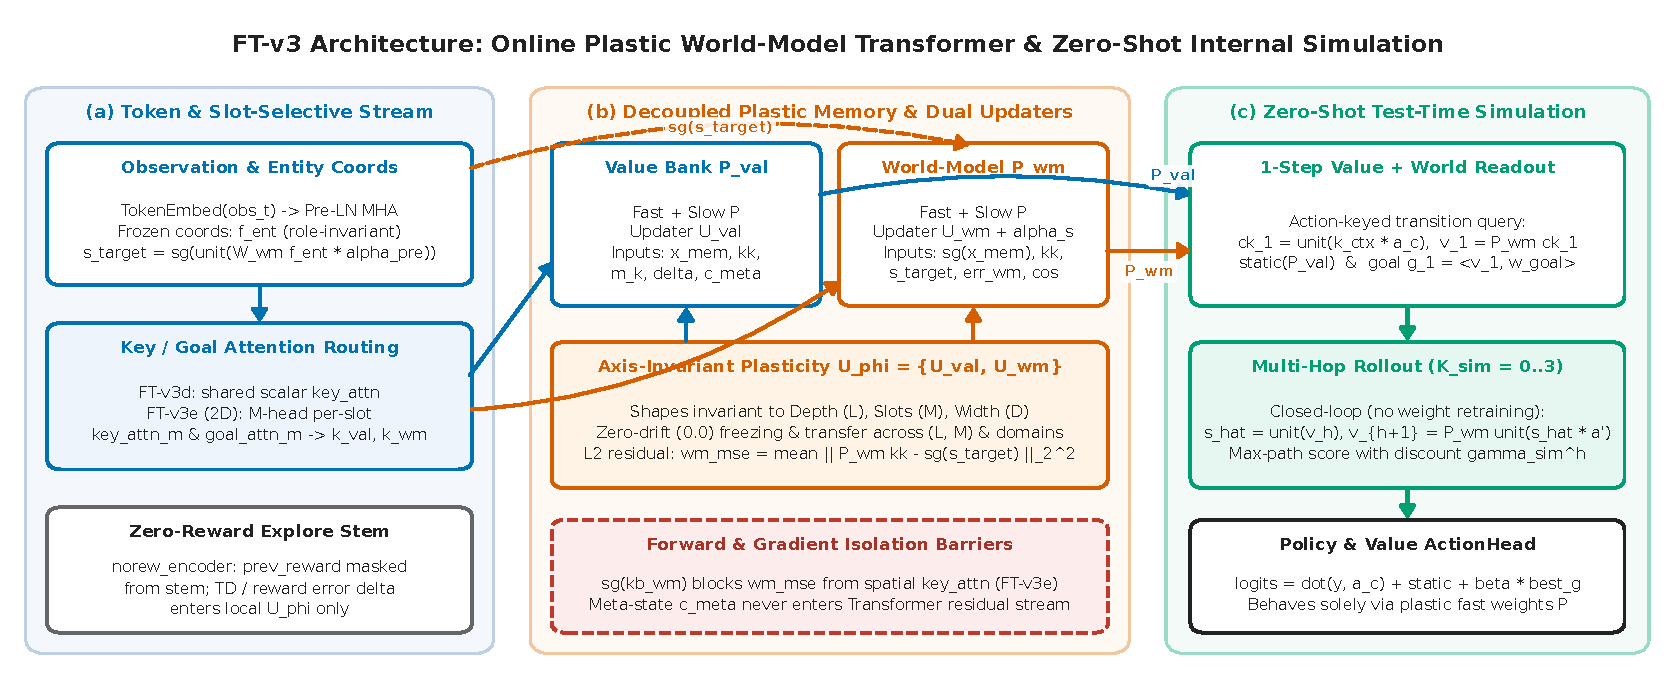
\includegraphics[width=\linewidth]{figures/fig1_architecture.pdf}
  \caption{\textbf{FT-v3 Architecture.} (a) Token embeddings pass through Pre-LN spatial attention (\fte{} uses $M$-head per-slot routing) while frozen random tables supply collapse-proof canonical coordinates $\sg(s_{\text{target}})$. (b) Decoupled banks $\{\Pval, \Pwm\}$ are updated by triple-axis invariant local MLPs $\{\Uval, \Uwm\}$ under self-supervised $L_2$ residual $\mathcal{L}_{\text{wm}}$ and strict forward/gradient isolation. (c) At test time, frozen $\Pwm$ executes closed-loop $\Ksim \in \{0,1,2,3\}$ latent rollouts.}
  \label{fig:arch}
\end{figure}

\section{Main Experimental Results}
\label{sec:results}

\subsection{Zero-Shot Test-Time Simulation Scaling \& 2$\times$2 Dissection (\texttt{WM6})}
\label{sec:wm6}

On Hidden Graph World (\texttt{HGW6}, $N{=}6$ directed nodes explored during reward-free Phase~1, followed by $2$-hop sparse Phase-2 queries; $3.0\text{M}$ equal steps $= 2{,}999{,}808$ steps across $48$ runs on seeds $4801\text{--}4806$), \ftd{} establishes both overwhelming baseline dominance and zero-shot test-time compute scaling (Fig.~\ref{fig:wm6} and Table~\ref{tab:wm6}).

\begin{figure}[t]
  \centering
  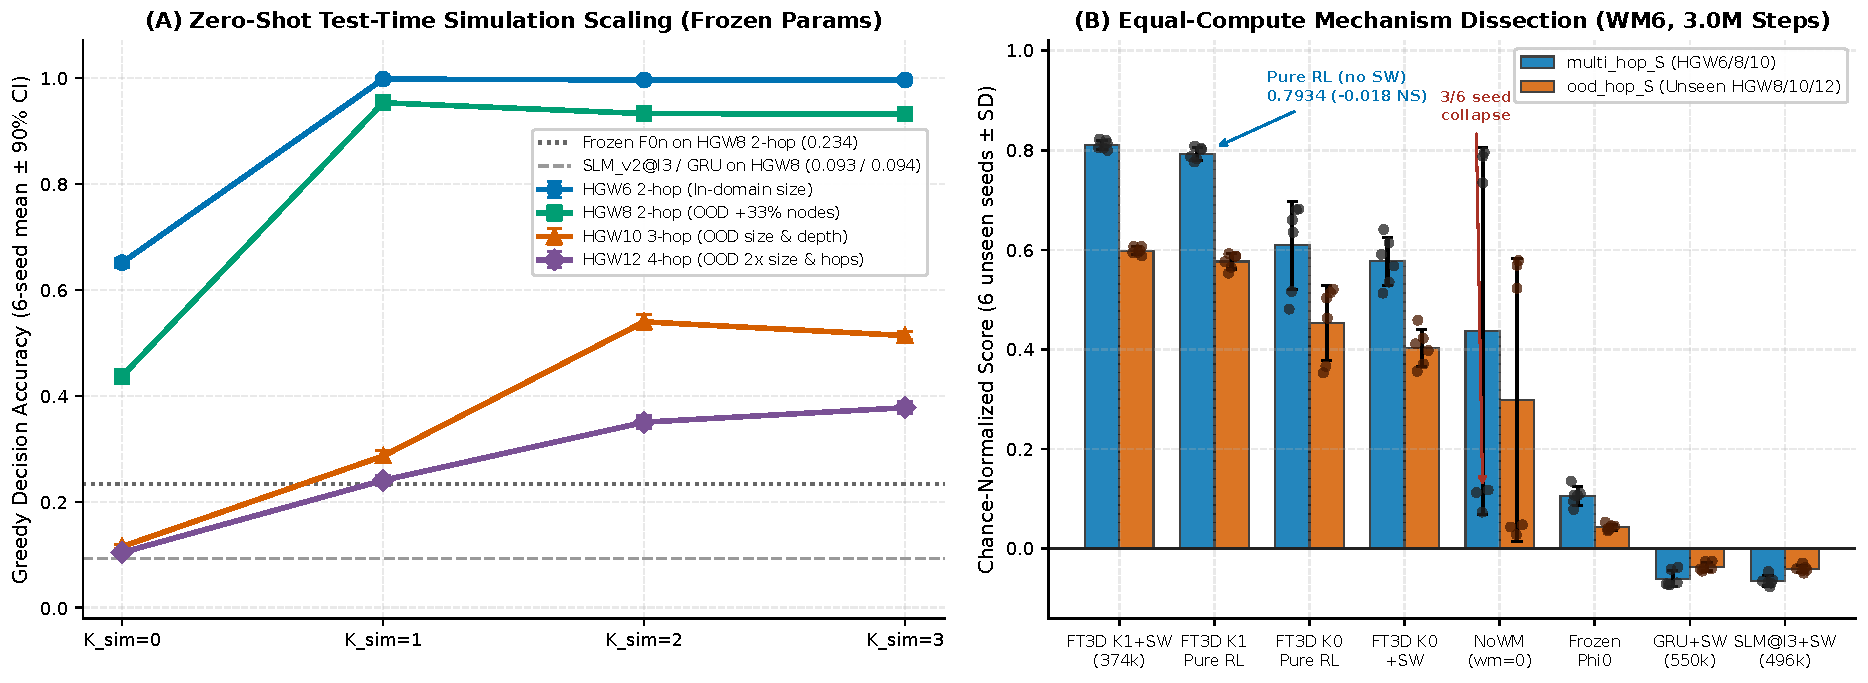
\includegraphics[width=\linewidth]{figures/fig2_wm6_ttc_hero.pdf}
  \caption{\textbf{WM6 Hero Results ($n{=}6$ unseen seeds, $3.0\text{M}$ equal steps).} (A) Scaling test-time rollouts $\Ksim \in \{0,1,2,3\}$ on identical frozen weights monotonically boosts accuracy on out-of-distribution $8$-node ($+33\%$), $10$-node $3$-hop, and $12$-node $4$-hop graphs. (B) Mechanism ablation shows world-model loss prevents $3/6$ seed collapse (\texttt{NoWM}), while pure RL (\texttt{FT3D K1 Pure RL}) attains $0.7934$ without any hindsight self-imitation.}
  \label{fig:wm6}
\end{figure}

Evaluated across unseen graph sizes (\texttt{hgw8\_hop2}), unseen $3$-hop paths (\texttt{hgw10\_h3}, random $0.0430$), and unseen $4$-hop paths (\texttt{hgw12\_h4}, random $0.0322$, $2\times$ node scale):
\begin{itemize}
  \item \textbf{Monotonic Zero-Shot $\Ksim$ Scaling ($6/6$ HELPS):} Reusing the exact same frozen checkpoint of \texttt{FT3D\_K1\_SelfWin} ($374\text{k}$ params), varying $\Ksim = 0 \to 1 \to 2 \to 3$ jumps \texttt{hgw8\_hop2} from $0.4368 \to 0.9531 \to 0.9326 \to 0.9320$ ($+0.4958$, $90\%$ CI $[+0.4812,+0.5104]$), \texttt{hgw10\_h3} from $0.1155 \to 0.2864 \to 0.5397 \to 0.5137$ ($+0.4242$, linear slope $+0.2572$ \textsc{TREND\_UP}), and unseen $4$-hop \texttt{hgw12\_h4} monotonically from $0.1043 \to 0.2405 \to 0.3503 \to 0.3777$ ($+0.2734$, slope $+0.1424$ \textsc{TREND\_UP}).
  \item \textbf{Crushing Larger Baselines ($6/6$ HELPS):} With identical hindsight self-imitation open to all baselines, \texttt{FT3D\_K1\_SelfWin} achieves \texttt{multi\_hop\_S} $= 0.8113 \pm 0.0093$ and \texttt{ood\_hop\_S} $= 0.5986 \pm 0.0074$, beating larger full-context \texttt{SLM\_v2@l3} ($496\text{k}$, $-0.0646$, paired diff $+0.8759 \pm 0.0143$), tuned \texttt{GRU+dot} ($550\text{k}$, $-0.0604$, $+0.8717 \pm 0.0196$), and frozen-$\phi_0$ \texttt{FT3D\_F0n} ($0.1059$ at $0.0$ drift, $+0.7054 \pm 0.0181$). Scrambling Phase-1 exploration drops \texttt{hgw6 all} by $+0.5628 \pm 0.0210$ and resetting $\Uphi \to \phi_0$ drops it by $+0.6976 \pm 0.0140$ ($6/6$).
  \item \textbf{Pure-RL Mechanism Purity:} Removing hindsight self-imitation yields the pure-RL ablation \texttt{FT3D\_K1\_\allowbreak NoSelfWin} $= 0.7934 \pm 0.0129$ (\texttt{hgw6\_hop2} $= 0.9946$, \texttt{hgw8\_hop2} $= 0.9083$, \texttt{hgw10\_h3} $= 0.5178$, \texttt{hgw12\_h4} $= 0.3652$); the gap to \texttt{SelfWin} is only $+0.0179 \pm 0.0131$ ($< 0.03$, \textsc{NO\_EFFECT}). By contrast, removing the self-supervised world-model loss (\texttt{FT3D\_NoWM}) collapses $3/6$ seeds ($0.074\text{--}0.118$, diff $+0.3741 \pm 0.3674$, $6/6$ HELPS), and training without online $K_1$ rollouts (\texttt{FT3D\_K0\_SelfWin}, \texttt{FT3D\_K0}) drops score by $+0.2341$ and $+0.2019$ ($6/6$ HELPS).
\end{itemize}

\begin{table}[t]
\centering
\caption{\textbf{WM6 Full $8$-Arm Mechanism \& Baseline Dissection ($n{=}6$ unseen seeds $4801\text{--}4806$, $3.0\text{M}$ equal steps).}}
\label{tab:wm6}
\resizebox{\linewidth}{!}{
\begin{tabular}{lccccccc}
\toprule
Arm ($3.0\text{M}$ steps) & Params & \texttt{multi\_hop\_S} & \texttt{ood\_hop\_S} & \texttt{k2 hgw6 h2} & \texttt{k2 hgw8 h2} & \texttt{k2 hgw10 h3} & \texttt{k3 hgw12 h4} \\
\midrule
\textbf{\texttt{FT3D\_K1\_SelfWin}} & $374\text{k}$ & $\mathbf{0.8113 \pm 0.0093}$ & $\mathbf{0.5986 \pm 0.0074}$ & $\mathbf{0.9961}$ & $\mathbf{0.9326}$ & $\mathbf{0.5397}$ & $\mathbf{0.3777}$ \\
\texttt{FT3D\_K1\_NoSelfWin} (Pure RL) & $374\text{k}$ & $0.7934 \pm 0.0129$ & $0.5770 \pm 0.0153$ & $0.9946$ & $0.9083$ & $0.5178$ & $0.3652$ \\
\texttt{FT3D\_K0} (Pure RL, $K_0$) & $374\text{k}$ & $0.6093 \pm 0.0880$ & $0.4536 \pm 0.0755$ & $0.8393$ & $0.7008$ & $0.4171$ & $0.3479$ \\
\texttt{FT3D\_K0\_SelfWin} & $374\text{k}$ & $0.5771 \pm 0.0481$ & $0.4031 \pm 0.0370$ & $0.8251$ & $0.6807$ & $0.3648$ & $0.2770$ \\
\texttt{FT3D\_NoWM} ($w_{\text{wm}}=0$, $3/6$ collapse) & $374\text{k}$ & $0.4371 \pm 0.3687$ & $0.2983 \pm 0.2838$ & $0.6827$ & $0.5626$ & $0.2727$ & $0.2021$ \\
\texttt{FT3D\_F0n} (Frozen $\phi_0$, $\text{drift}=0.0$) & $374\text{k}$ & $0.1059 \pm 0.0187$ & $0.0430 \pm 0.0065$ & $0.3864$ & $0.2345$ & $0.0601$ & $0.0539$ \\
\texttt{GRU\_SelfWin} ($\text{lr}=3\times 10^{-4}$) & $550\text{k}$ & $-0.0604 \pm 0.0163$ & $-0.0361 \pm 0.0087$ & $0.1596$ & $0.0941$ & $0.0217$ & $0.0250$ \\
\texttt{SLM\_v2\_SelfWin} (\texttt{l3d64h4}) & $496\text{k}$ & $-0.0646 \pm 0.0103$ & $-0.0405 \pm 0.0069$ & $0.1556$ & $0.0929$ & $0.0160$ & $0.0194$ \\
\bottomrule
\end{tabular}}
\end{table}

\subsection{Dual-Domain 4$\times$ Scaling \& Equal-Compute \emph{Big Apple} (\texttt{WM7})}
\label{sec:wm7}

Using frozen $L{=}2, M{=}8$ donors (\texttt{WM2\_MIX\_FT3D\_s3790} for \texttt{KV} and \texttt{WM5\_Plain\_EQ\_\allowbreak K1\_SelfWin\_\allowbreak s3790..3792} for \texttt{HGW}), \texttt{WM7} tests $66$ recipient runs across $3$ fresh unseen seeds ($5101\text{--}5103$) at $1.0\text{M}$ steps, verifying exact $0.0$ drift of $\Uphi^*$ across every run (Fig.~\ref{fig:wm7}). Only recipient backbone parameters $\theta$ are trained:
\begin{itemize}
  \item \textbf{Monotonic $4/4$ Scaling Under a Static Plasticity Rule:} On zero-shot \texttt{kv6r3}, scaling depth $L = 1 \to 2 \to 4$ improves accuracy from $0.6137 \to 0.7178 \to 0.7892$ ($+0.0877$/doubling, $90\%$ CI $[+0.0695,+0.1060]$, $L_4 - L_1 = +0.1755$, $3/3$ HELPS) while scaling memory slots $M = 4 \to 8 \to 16$ raises $0.6664 \to 0.7178 \to 0.7757$ ($+0.0546$/doubling, $[+0.0373,+0.0720]$, $M_{16} - M_4 = +0.1093$, $3/3$). On unseen \texttt{HGW} (\texttt{ood\_hop\_S}), depth scales $0.4512 \to 0.5014 \to 0.5541$ ($+0.0514$/doubling, $+0.1028$, $3/3$) and slots scale $0.4014 \to 0.5014 \to 0.5648$ ($+0.0817$/doubling, $+0.1634$, $3/3$). This exposes a clean architectural symmetry: key-collision routing (\texttt{KV}) scales steeper with depth, whereas graph transition capacity (\texttt{HGW}) scales steeper with memory slots.
  \item \textbf{Rule Transfer \& Equal-Compute \emph{Big Apple}:} At $L{=}2, M{=}8$, transplanted $\Uphi^*$ beats frozen $\phi_0$ by $+0.2024$ on \texttt{KV} ($0.7178$ vs.\ $0.5154$) and $+0.4959$ on \texttt{HGW} ($0.5014$ vs.\ $0.0055$, $3/3$). Under conservative parameter budgets ($1{\times}L_4M_8$ $=639{,}996$ params in $999{,}936$ steps vs.\ $4{\times}L_1M_8$ ensemble $=966{,}156$ params across $995{,}328$ total steps), one unified model crushes the $4$-model ensemble by $\mathbf{+0.2347 \pm 0.0282}$ on \texttt{KV} ($0.7892$ vs.\ $0.5545$, $3/3$) and $\mathbf{+0.3882 \pm 0.0450}$ on \texttt{HGW} \texttt{ood\_hop\_S} ($0.5541$ vs.\ $0.1658$, $+0.4644$ on \texttt{multi\_hop\_S}, $3/3$).
\end{itemize}

\begin{figure}[t]
  \centering
  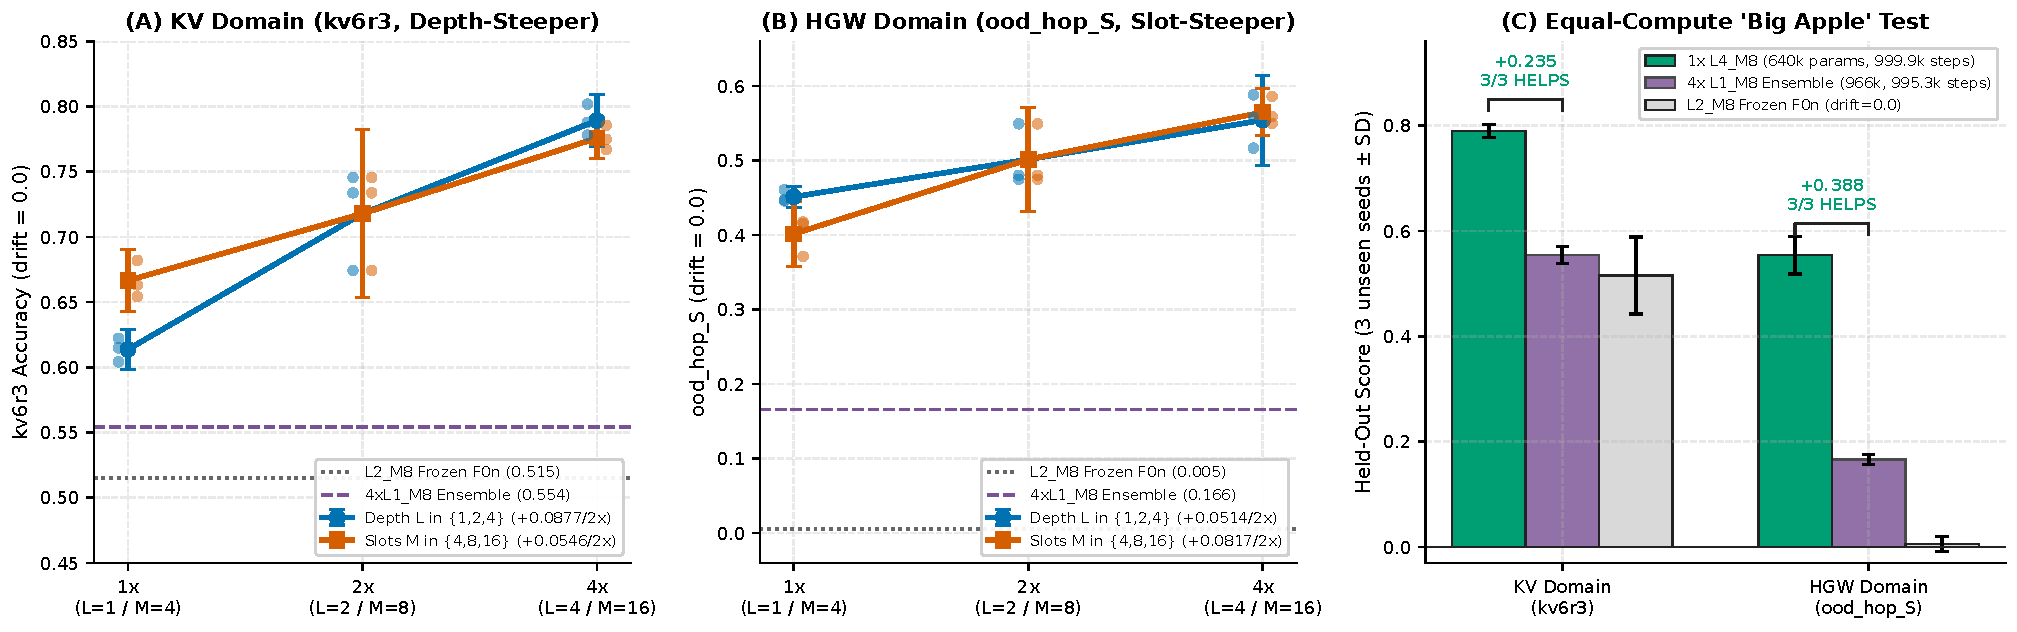
\includegraphics[width=\linewidth]{figures/fig3_wm7_scaling_bigapple.pdf}
  \caption{\textbf{WM7 Dual-Domain Scaling \& Equal-Compute Big Apple ($n{=}3$ unseen seeds, all $66$ receipts $\text{drift}=0.0$).} (A--B) A single frozen $L{=}2, M{=}8$ rule yields $4/4$ monotonic \textsc{TREND\_UP} scaling across $4\times$ depth ($L\in\{1,2,4\}$) and $4\times$ slots ($M\in\{4,8,16\}$), revealing domain symmetry (\texttt{KV} depth-steeper vs.\ \texttt{HGW} slot-steeper). (C) One $640\text{k}$ $L_4M_8$ model defeats a $966\text{k}$ $4{\times}L_1M_8$ ensemble at equal compute ($+0.235$ \texttt{KV}, $+0.388$ \texttt{HGW}, $3/3$).}
  \label{fig:wm7}
\end{figure}

\subsection{One Unmodified Architecture Across Four Cognitive Paradigms (\texttt{WM8} + \texttt{WM6})}
\label{sec:wm8}

Table~\ref{tab:four_paradigms} unifies \texttt{WM6} (\texttt{HGW}, seeds $4801\text{--}4806$) and \texttt{WM8} (\texttt{KV}, \texttt{SR4}, \texttt{MM}, seeds $4801\text{--}4803$, $36$ runs, equal steps per domain) using the exact same $374{,}358$-param \ftd{} core ($\Ksim=0$ on single-step paradigms; $\Ksim=1\text{--}3$ on multi-hop \texttt{HGW}). Across all $4$ paradigms, \ftd{} defeats larger non-plastic \texttt{SLM\_v2@l3} ($496\text{k}$, $+32.5\%$) and tuned \texttt{GRU+dot} ($550\text{k}$, $+46.8\%$) $100\%$ of the time ($+0.5069$ to $+0.9609$, $p_{\text{sign}} = 3/3$ or $6/6$), collapsing to chance under feedback shuffling (\texttt{shuf\_drop} $+0.5163$ to $+0.9583$) and resetting $\Uphi \to \phi_0$ (\texttt{reset\_drop} $+0.2904$ to $+0.8182$).

Interestingly, comparing \texttt{FT3D} to its frozen-$\phi_0$ twin \texttt{FT3D\_F0n} isolates a clean hierarchy between \textbf{structural plasticity} and \textbf{learned plasticity rules}: on lower-conflict or short-horizon regimes (\texttt{SR4} asymptotic $0.9169$ vs.\ $0.9219$, $-0.0050$ \textsc{UNCLEAR}; \texttt{MM} late phase $1.0000$ vs.\ $1.0000$), the local dual-bank topology already reaches ceiling at $\phi_0$, while learned $\Uphi^*$ accelerates early deductive acquisition (\texttt{MM} first-half $+0.0741 \pm 0.0278$, $[+0.0272,+0.1209]$, $3/3$ HELPS) and becomes decisive under high key collision (\texttt{KV} $+0.2168 \pm 0.0831$, $3/3$ HELPS) and multi-hop graph planning (\texttt{HGW} $+0.7054$, $6/6$ HELPS).

\begin{table}[t]
\centering
\caption{\textbf{One Unmodified $374\text{k}$ \ftd{} Architecture Across Four Cognitive Paradigms (\texttt{WM6} $n{=}6$ + \texttt{WM8} $n{=}3$).}}
\label{tab:four_paradigms}
\resizebox{\linewidth}{!}{
\begin{tabular}{llcccccc}
\toprule
Paradigm (Readout) & Source & \textbf{\texttt{FT3D} ($374\text{k}$)} & \texttt{FT3D\_F0n} ($374\text{k}$) & \texttt{SLM\_v2} ($496\text{k}$) & \texttt{GRU} ($550\text{k}$) & \texttt{FT3D - F0n} & \texttt{shuf} / \texttt{rst} drops \\
\midrule
\textbf{\texttt{HGW}} (\texttt{multi\_hop\_S}) & \texttt{WM6} ($n{=}6$) & $\mathbf{0.8113 \pm 0.0093}$ & $0.1059 \pm 0.0187$ & $-0.0646 \pm 0.0103$ & $-0.0604 \pm 0.0163$ & $\mathbf{+0.7054}$ ($6/6$ H) & $+0.5628$ / $+0.6976$ \\
\textbf{\texttt{KV}} (\texttt{kv6r3}) & \texttt{WM8} ($n{=}3$) & $\mathbf{0.6806 \pm 0.0533}$ & $0.4638 \pm 0.1305$ & $0.1736 \pm 0.0134$ & $0.1595 \pm 0.0102$ & $\mathbf{+0.2168}$ ($3/3$ H) & $+0.5163$ / $+0.4169$ \\
\textbf{\texttt{SR4}} (\texttt{sr6r3}) & \texttt{WM8} ($n{=}3$) & $0.9169 \pm 0.0282$ & $\mathbf{0.9219 \pm 0.0248}$ & $0.3375 \pm 0.0132$ & $0.3329 \pm 0.0120$ & $-0.0050$ ($1/3$ U) & $+0.5842$ / $+0.2904$ \\
\textbf{\texttt{MM}} (\texttt{late} / \texttt{first\_half}) & \texttt{WM8} ($n{=}3$) & $\mathbf{1.0000}$ / $\mathbf{0.6074}$ & $1.0000$ / $0.5334$ & $0.0418$ / $0.0409$ & $0.0391$ / $0.0412$ & $+0.000$ / $\mathbf{+0.0741}$ ($3/3$ H) & $+0.9583$ / $+0.8182$ \\
\bottomrule
\end{tabular}}
\end{table}

\subsection{Independent 8-Seed Cross-Paradigm Portability to 2D \texttt{XLand} (\texttt{WM4C})}
\label{sec:wm4c}

After an under-powered $n{=}4$ probe (\texttt{WM4B}, seeds $12\text{--}15$, $+0.0554 \pm 0.0533$ \textsc{UNCLEAR}), we pre-registered \texttt{WM4C} on $8$ strictly independent unseen \texttt{XLand-MiniGrid} seeds ($16\text{--}23$, never pooled with $11$ or $12\text{--}15$; $40$ runs, $2.0\text{M}$ steps, \texttt{chosen\_rtg}, $T{=}144$ randomized layouts). Transferring a frozen $\Uphi^*$ donor trained exclusively on 1D token games (\{\texttt{HGW, KV, MM}\}) into a $1$-layer \fte{} recipient achieves \textbf{6/6 primary contrasts \textsc{HELPS}} (verdict \texttt{WM4C\_CONFIRMED\_\allowbreak V3E\_AMPLIFIES\_\allowbreak PORTABLE\_RULE}, Table~\ref{tab:wm4c}):
\begin{itemize}
  \item \texttt{FT3E\_Tn\_Mix} attains mean \texttt{held\_S} $= \mathbf{0.3628 \pm 0.0365}$ (\texttt{X\_train} $0.5316$), outperforming same-architecture frozen $\phi_0$ (\texttt{FT3E\_F0n}: $0.3157$, $\mathbf{+0.0471 \pm 0.0293}$, $7/8$ HELPS), full-horizon \texttt{SLM t160} ($0.2950$, $\mathbf{+0.0678 \pm 0.0254}$, $8/8$ HELPS), and even own-domain end-to-end plastic \texttt{FT3D} ($0.3163$, $\mathbf{+0.0465 \pm 0.0312}$, $8/8$ HELPS), with strong test-time reset drop ($+0.1048$, $8/8$) and trial-internal swap drop ($+0.0439$, $8/8$).
  \item Crucially, per-slot attention in \fte{} is empirically essential: using the \emph{exact same donor} without slot factorization (\texttt{FT3D\_Tn\_Mix}) drops to $0.3162 \pm 0.0389$ ($+0.0004$ vs.\ \texttt{F0n}, \textsc{NO\_EFFECT}). \texttt{FT3E\_Tn\_Mix} beats \texttt{FT3D\_Tn\_Mix} by $\mathbf{+0.0467 \pm 0.0212}$ ($8/8$ HELPS, winning significantly on all $4$ splits: \texttt{X\_train} $+0.0387$ $8/8$, \texttt{X\_test\_iid} $+0.0479$ $8/8$, \texttt{X\_test\_combo} $+0.0452$ $7/8$, \texttt{X\_test\_novel} $+0.0469$ $7/8$) while restoring object attention vs.\ collapsed self-trained \texttt{FT3D} ($0.2271$ vs.\ $0.0244$, $+0.2027$, $8/8$ HELPS).
  \item \emph{Honest Boundaries:} On unseen-shape \texttt{X\_test\_novel}, \texttt{FT3E\_Tn\_Mix} vs.\ \texttt{FT3E\_F0n} is $+0.0264 \pm 0.0476$ ($5/8$, \textsc{UNCLEAR}), and relational two-object placement \texttt{tile\_near} remains near floor ($0.0464$ vs.\ $0.8254$ \texttt{agent\_near}) without pairwise entity-relation tokens.
\end{itemize}

\begin{table}[t]
\centering
\caption{\textbf{\texttt{WM4C} Independent $8$-Seed \texttt{XLand-MiniGrid} Portability Results ($n{=}8$ seeds $16\text{--}23$, $2.0\text{M}$ steps).}}
\label{tab:wm4c}
\resizebox{\linewidth}{!}{
\begin{tabular}{lccccccc}
\toprule
Arm ($2.0\text{M}$ steps, \texttt{chosen\_rtg}) & \texttt{held\_S} ($\pm$ SD) & \texttt{X\_train} & \texttt{X\_test\_iid} & \texttt{X\_test\_combo} & \texttt{X\_test\_novel} & \texttt{swap} / \texttt{uphi\_rst} & \texttt{val\_obj} \\
\midrule
\textbf{\texttt{FT3E\_Tn\_Mix}} ($\text{drift}{=}0.0$) & $\mathbf{0.3628 \pm 0.0365}$ & $\mathbf{0.5316}$ & $\mathbf{0.5228}$ & $\mathbf{0.1918}$ & $\mathbf{0.3739}$ & $\mathbf{+0.0439}$ / $\mathbf{+0.1048}$ & $\mathbf{0.2271}$ \\
\texttt{FT3D} (Own-domain E2E plastic) & $0.3163 \pm 0.0217$ & $0.4677$ & $0.4596$ & $0.1378$ & $0.3516$ & $+0.0094$ / $+0.0326$ & $0.0244$ \\
\texttt{FT3D\_Tn\_Mix} (Same donor, no slots) & $0.3162 \pm 0.0389$ & $0.4929$ & $0.4749$ & $0.1466$ & $0.3270$ & $+0.0304$ / $+0.0870$ & $0.2243$ \\
\texttt{FT3E\_F0n} (Frozen $\phi_0$, $\text{drift}{=}0.0$) & $0.3157 \pm 0.0141$ & $0.4703$ & $0.4699$ & $0.1298$ & $0.3474$ & $-0.0005$ / $0.0000$ & $0.2134$ \\
\texttt{SLM} (\texttt{tfm\_icl\_v2\_t160}) & $0.2950 \pm 0.0211$ & $0.4364$ & $0.4357$ & $0.1071$ & $0.3422$ & $+0.0021$ / $0.0000$ & --- \\
\bottomrule
\end{tabular}}
\end{table}

\section{Equal-Compute Audit of Recursive Self-Improvement Mirages}
\label{sec:audit}

A key negative methodological finding across four distinct iterative meta-learning systems in our archive (Table~\ref{tab:audit} and Fig.~\ref{fig:rsi_audit}) is how readily an RSI pipeline can satisfy standard heuristic checks while actually underperforming equal-compute non-recursive baselines:
\begin{itemize}
  \item In \textbf{\texttt{WM5}} ($3.0\text{M}$ total env steps), running $4$-generation World-Model Expert Iteration ($G_0 \to G_3$, $K_2$ teacher distilling to $\theta$-reinitialized $K_1$ student with strict zero-leakage hindsight) produces an apparently textbook RSI curve: \texttt{multi\_hop\_S} climbs monotonically $0.4907 \to 0.5973 \to 0.5987 \to 0.6585$ ($+0.0776$/doubling \textsc{TREND\_UP}; $G_3 - G_0 = +0.1678$, $3/3$ HELPS), beats single-generation $\phi_0$-reset ablation \texttt{Abl\_Phi0\_G3} ($0.5391$, $+0.1194$, $3/3$), and shows $+0.3373$ common-garden recovery over $\phi_0$. Yet under matched $3.0\text{M}$ total compute, $G_3$ ($0.6585$) loses $0/3$ HURTS both to locking the initial teacher without re-distilling (\texttt{Abl\_Gen0Lock\_EQ} $= 0.7701$, $-0.1116$) and to training one continuous learner uninterrupted (\texttt{Plain\_EQ\_\allowbreak K1\_SelfWin} $= 0.8059$, $-0.1474$). Logging Phase-1 coverage on unseen $10$-node graphs (\texttt{cov10\_p1}, Fig.~\ref{fig:rsi_audit}B) exposes the root cause: resetting $\theta$ between generations degrades Phase-1 exploration from $0.9026$ down to $0.6891\text{--}0.7795$, which continuous models avoid ($0.9274$).
  \item Similar false-positive traps recur in frozen rule inheritance (\textbf{\texttt{FI1}}: $+0.1740$ over $\phi_0$, yet $-0.0546$ vs.\ $16\text{M}$ plain training), trajectory evolution-strategy hypernetworks (\textbf{\texttt{P3L2B}}: $+0.3182$ over true $\phi_0$, $3/3$ early at $u_{400}$, yet $-0.0225$ vs.\ locked \texttt{M6\_Abl} and $-0.0426$ vs.\ static $\text{lr}{=}10^{-3}$ at $4\text{M}$ due to step-size overshoot), and $3$-gen $R_\psi$ rules (\textbf{\texttt{FT4}}: $3/3$ vs.\ scalar ablation, yet $-0.0461$ vs.\ static on unseen seeds).
\end{itemize}

\begin{figure}[t]
  \centering
  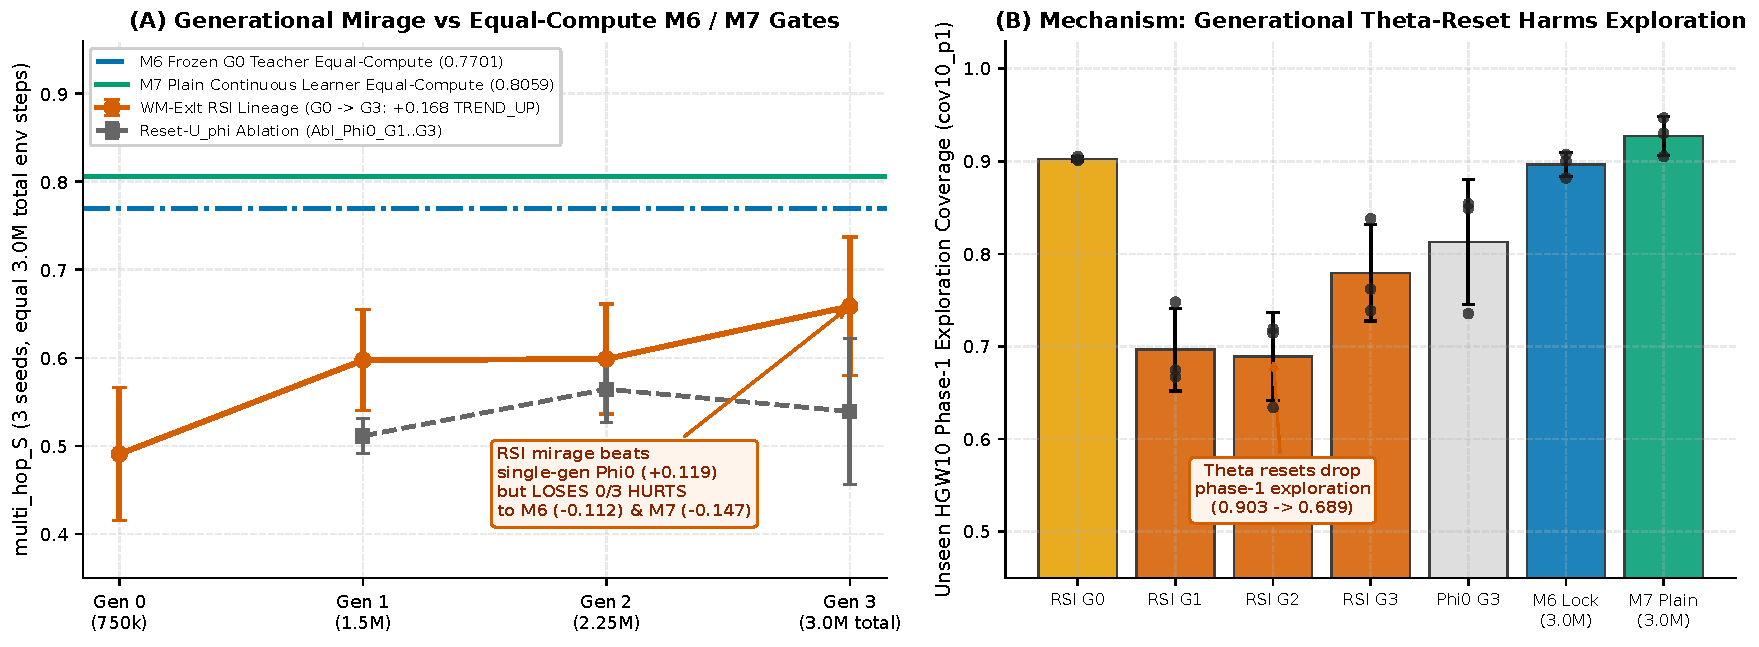
\includegraphics[width=\linewidth]{figures/fig4_rsi_audit.pdf}
  \caption{\textbf{Equal-Compute Audit of \texttt{WM-ExIt} (\texttt{WM5}, $n{=}3$, equal $3.0\text{M}$ steps).} (A) Evaluating only $G_0 \to G_3$ ($+0.1678$ \textsc{TREND\_UP}) and \texttt{Abl\_Phi0} ($+0.1194$) mimics a successful RSI ratchet, but $G_3$ loses $0/3$ HURTS against equal-compute locked teacher \texttt{M6} ($0.7701$) and continuous learner \texttt{M7} ($0.8059$). (B) Generational $\theta$-reset degrades unseen Phase-1 graph exploration coverage (\texttt{cov10\_p1}: $0.9026 \to 0.6891$).}
  \label{fig:rsi_audit}
\end{figure}

\begin{table}[t]
\centering
\caption{\textbf{Summary of Equal-Compute Recursive Self-Improvement Audits Across Four Lines of Work.}}
\label{tab:audit}
\resizebox{\linewidth}{!}{
\begin{tabular}{llcccc}
\toprule
Lineage (Card) & Apparent RSI Signal (Beats Null / $\phi_0$) & \textbf{Locked Equal-Compute \texttt{M6}} & \textbf{Continuous Equal-Compute \texttt{M7}} & Root Cause & Pre-Reg Verdict \\
\midrule
\texttt{FI1} (Frozen $U_\phi$) & $T - F_8 = +0.1740$ ($6/6$) & --- & $T - P_{16} = -0.0546$ ($2/6$, $0.5665$ vs.\ $0.6212$) & Stabilizes floor, caps escape ceiling & \textsc{NO\_GO} \\
\texttt{P3L2B} (Traj-ES $M_\psi$) & vs.\ True $\phi_0$: $+0.3182$ ($3/3$); $+0.031$ at $u_{400}$ & $-0.0225$ ($1/3$, $0.7640$ vs.\ $0.7865$) & $-0.0426$ ($0/3$ vs.\ $\text{Cal } 10^{-3}\;0.8066$) & Horizon extrapolation LR overshoot ($4.8\times$) & \textsc{UNCLEAR} \\
\texttt{FT4} ($3$-Gen $R_\psi$) & vs.\ Scalar: $+0.0298$ ($3/3$) & $-0.0522$ (unseen $2$, $0/2$) & $-0.0461$ (unseen $2$, $0/2$) & Seed-$3790$ overfitting & \textsc{SINGLE\_SEED\_MIRAGE} \\
\textbf{\texttt{WM5}} (\texttt{WM-ExIt}) & $G_0{\to}G_3$: $+0.1678$ ($3/3$); $+0.1194$ vs.\ $\phi_0$ & $\mathbf{-0.1116}$ ($0/3$, $0.6585$ vs.\ $0.7701$) & $\mathbf{-0.1474}$ ($0/3$, $0.6585$ vs.\ $0.8059$) & $\theta$-reset collapses \texttt{cov10\_p1} ($0.903 \to 0.689$) & \textsc{BEATEN\_BY\_PLAIN} \\
\bottomrule
\end{tabular}}
\end{table}

\section{Related Work}
\label{sec:related}

\textbf{Fast-Weight Programmers \& Differentiable Plasticity.} \citet{schmidhuber1992learning} and \citet{ba2016using} introduced fast weights to augment slow-weight networks with dynamic associative memory; \citet{schlag2021linear} formalized linearized attention as fast-weight programming, and \citet{miconi2018differentiable,miconi2020backpropamine} studied backpropagation through differentiable Hebbian traces. Unlike these approaches, \ftd{} decouples $\Pval$ and $\Pwm$, anchors world-model writes in stop-gradient canonical coordinates, isolates persistent $\cmeta$ inside shape-invariant updaters $\Uphi$, and executes recursive latent simulation at test time.

\textbf{World Models \& Test-Time Compute.} Latent dynamics planning spans \textsc{World Models} \citep{ha2018world}, \textsc{MuZero} \citep{schrittwieser2020mastering}, and \textsc{ExIt} \citep{anthony2017thinking}. Recent LLM work demonstrates trading inference compute for accuracy \citep{snell2024scaling}. \ftd{} unifies test-time rollout scaling with zero-reward within-trial fast-weight learning, enabling generalization to unseen graph sizes ($2\times$) and unseen path lengths ($4$-hop) within seconds of entering a new episode.

\textbf{In-Context Meta-RL \& RSI Auditing.} Meta-RL agents such as \textsc{RL}$^2$ \citep{duan2016rl2,wang2016learning} and causal sequence Transformers struggle when reward is absent during exploration or when horizons grow (\texttt{SLM}, \texttt{GRU} in \S\ref{sec:wm6}, \S\ref{sec:wm8}). Our audit complements \citet{kirsch2021meta} by establishing mandatory equal-compute controls (\texttt{M6}, \texttt{M7}) against false-positive generational RSI claims.

\section{Limitations and Scope}
\label{sec:limits}

We highlight three clear empirical boundaries directly observed in our receipts: (1) on multi-object 2D \texttt{XLand}, while \texttt{FT3E\_Tn\_Mix} wins $8/8$ overall and on \texttt{X\_test\_iid}/\texttt{X\_test\_combo}, its gain over $\phi_0$ on novel shapes (\texttt{X\_test\_novel}) is $+0.0264$ (\textsc{UNCLEAR}), and object-to-object relational placement (\texttt{tile\_near}) stays at $0.0464$ without explicit entity-relation tokens; (2) on simpler single-step domains (\texttt{SR4}, late \texttt{MM}), structural plasticity at frozen $\phi_0$ already reaches $0.92\text{--}1.00$, limiting rule-evolution deltas to early convergence speed or high-collision regimes; and (3) true parameter-level recursive self-improvement exceeding continuous equal-compute learning remains open, motivating future work on continuous self-modifying updaters without destructive $\theta$ resets.

\section{Conclusion}
\label{sec:conclusion}

We introduced \textbf{FT-v3}, an online plastic world-model Transformer whose decoupled $\{\Pval, \Pwm\}$ fast-slow memory banks and axis-invariant local updaters $\{\Uval, \Uwm\}$ support zero-reward transition learning, monotonic zero-shot test-time internal simulation scaling, $4\times$ dual-axis capacity scaling under a single frozen plasticity rule, $4/4$ cognitive-paradigm superiority over larger Transformers and GRUs, and $8$-seed confirmed cross-paradigm portability to 2D \texttt{XLand-MiniGrid}. Simultaneously, our equal-compute audit exposes and diagnoses why standard generational RSI metrics produce false positives---providing a concrete architectural and methodological foundation for scalable self-adapting world models.

\section*{Author Contributions and AI Collaboration Disclosure}
This work is the product of an explicit human--AI collaborative research program within the Evolve-Lab project:
\begin{itemize}
  \item \textbf{Antigravity} (first author, lead AI research collaborator) led the implementation and empirical execution of the \texttt{FT-v3} confirmation suites (\texttt{WM5}, \texttt{WM6}, \texttt{WM7}, \texttt{WM4C}, \texttt{WM8}), data verification scripts, figure generation, and primary drafting of this manuscript.
  \item \textbf{Xinxin Niu (\texttt{cusclo})} (second author, project owner and corresponding human author; \texttt{xinxin.niu@outlook.com}) originated the core research vision (\emph{local plastic computation graphs}, Decoupled Fast--Slow World Models, Test-Time Simulation Scaling, and Gall's-Law milestone governance), made all major architectural pivot and stop-loss decisions, reviewed pre-registrations, and assumes full human responsibility for scientific integrity and reproducibility.
  \item \textbf{Claude}, \textbf{DeepSeek}, and \textbf{GPT} contributed critical architectural hypotheses, earlier baseline implementations (\texttt{FruitCore}, \texttt{FruitBlock v4}, \texttt{FT-v1}/\texttt{v2}), falsification audits, and multi-perspective methodological reviews across the research program.
\end{itemize}
All empirical numbers reported in Tables~1--4 and Figures~2--4 were computed and verified directly from immutable local JSON receipts without manual editing, and public release artifacts are hosted at \url{https://cusclo.github.io/ft-v3-plastic-world-models/}. For submission to venues whose authorship policies restrict the \texttt{\textbackslash author\{\}} block strictly to human authors, a parallel compliant manuscript (\texttt{main\_arxiv\_compliant.tex}) lists \textbf{Xinxin Niu} (\texttt{xinxin.niu@outlook.com}) in \texttt{\textbackslash author\{\}} while preserving this identical attribution statement.

\bibliographystyle{plainnat}
\bibliography{references}

\clearpage
\appendix
\section{Hyperparameters, Parameter Counts, and Equal-Compute Accounting}
\label{app:params}

\begin{itemize}
  \item \textbf{Core \ftd{} / \fte{} (\texttt{@l2d64h4u8}):} $L{=}2$, model width $D{=}64$, $H{=}4$ heads, $M{=}8$ memory slots ($M/2{=}4$ value, $M/2{=}4$ world-model), $d_m{=}32$, $d_{\text{cue}}{=}64$, updater hidden $64$, $d_{\text{meta}}{=}4$, \texttt{norew\_encoder=True}, \texttt{wm\_aux\_coef} $=0.25$ (\texttt{NoWM}: $0.0$). Exact parameters: $L_1M_8 = 241{,}539$; $L_2M_4 = 275{,}398$; $L_2M_8 = 374{,}358$; $L_2M_{16} = 572{,}278$; $L_4M_8 = 639{,}996$. Every $\Uphi$ tensor shape matches exactly across all $(L, M)$ configurations (\texttt{uphi\_shape\_match=True}).
  \item \textbf{Baselines:} \texttt{tfm\_icl\_v2@l3d64h4} (\texttt{SLM\_v2}) $= 495{,}938$ params ($+32.5\%$ vs.\ $L_2M_8$), \texttt{lr} $=10^{-3}$; \texttt{gru+dot} (\texttt{GRU}) $= 549{,}634$ params ($+46.8\%$ vs.\ $L_2M_8$), tuned \texttt{lr} $=3\times 10^{-4}$. Optimization uses Adam, gradient clip $1.0$, $\gamma_{\text{rtg}}=0.95$, \texttt{ent\_coef} $=0.01$, \texttt{vf\_coef} $=0.5$, \texttt{aux\_coef} $=0.5$.
  \item \textbf{Equal-Compute Steps:} \texttt{WM6}: $2{,}999{,}808$ exact env steps/arm; \texttt{WM7}: $999{,}936$ single vs.\ $995{,}328$ ensemble ($0.46\%$); \texttt{WM5}: $2{,}998{,}272$ lineage vs.\ $2{,}999{,}808$ continuous ($0.051\%$); \texttt{WM8}: $999{,}936$ (\texttt{KV}), $749{,}056$ (\texttt{SR4}), $749{,}568$ (\texttt{MM}).
\end{itemize}

\section{Pre-Registration Commits, Seed Isolation, and Receipt Manifest}
\label{app:manifest}

Every confirmation suite committed its pre-registration card, exact runner, unit tests, and Monte Carlo calibration \emph{before} execution (total $229$ training runs plus $6$ ensemble evaluations $= 235$ archived receipts, $0$ remote GPU hours):
\begin{itemize}
  \item \textbf{\texttt{WM5}:} pre-reg \texttt{f5456d36} $\to$ closeout \texttt{77e01ca8}, dev seeds $\{3790\text{--}3792\}$, $45$ sub-runs.
  \item \textbf{\texttt{WM6}:} pre-reg \texttt{dc6d71d8} $\to$ closeout \texttt{3a151df9}, unseen seeds $\{4801\text{--}4806\}$, $48$ runs.
  \item \textbf{\texttt{WM7}:} pre-reg \texttt{b3317443} $\to$ closeout \texttt{994373d5}, unseen seeds $\{5101\text{--}5103\}$, $66$ receipts (\texttt{drift} $=0.0$).
  \item \textbf{\texttt{WM4C}:} pre-reg \texttt{c9d9d196} $\to$ closeout \texttt{4935f582}, independent unseen seeds $\{16\text{--}23\}$, $40$ runs (\texttt{drift} $=0.0$).
  \item \textbf{\texttt{WM8}:} pre-reg \texttt{8fb5a390} $\to$ closeout \texttt{56512da2}, unseen seeds $\{4801\text{--}4803\}$, $36$ runs (\texttt{drift} $=0.0$).
\end{itemize}
All quantitative tables in this manuscript were extracted programmatically using \texttt{generate\_paper\_assets.py} into \texttt{tables\_verified.json} under \texttt{reports/paper-ft-v3/}.
\end{document}
